\section{Arithmetic determinant bounds with vanishing minors}
\label{sec:determinants}

The repository organizes its central comparison around short integral
forms, enough forms to span, and a lower bound saying that integral forms
are long; determinants combine these inputs
\cite{guide,mainineq}. This suggests an independent finite-dimensional
question. How small can an integer matrix's Gram determinant be when
many of its maximal minors are nonzero? Integrality gives one lower
bound, but the algebraic relations between minors force a stronger one.
The result below also quantifies what remains when some minors vanish.
It is unconditional and does not use RH.

\begin{theorem}[Arithmetic determinant amplification]
\label{thm:determinant}
Let $A\in\Z^{r\times n}$ have row rank $r$, where $n\ge5$ and
$2\le r\le n-2$. For an $r$-element subset $B\subseteq\{1,\ldots,n\}$,
write $A_B$ for the square matrix formed by its columns in increasing
order. Define
\[
 N=\binom nr,\qquad
 z=\#\{B:\det A_B=0\},\qquad
 D=\gcd\{\lvert\det A_B\rvert:\det A_B\ne0\}.
\]
Then $D>0$ and
\begin{equation}
\boxed{\quad
 \frac{\det(AA^{\mathsf T})}{D^2}
 \ge
 \max\left\{N-z,\ \frac85N-4z,\ \frac{12}5N-12z\right\}.
 \quad}
\label{eq:det-main}
\end{equation}
In particular, if every $r$ columns are linearly independent, then
\begin{equation}
 \det(AA^{\mathsf T})\ge\frac{12}{5}\binom nr D^2.
 \label{eq:det-generic}
\end{equation}
The coefficient $12/5$ in \eqref{eq:det-generic} cannot be increased
uniformly over this class. Each of the three affine inequalities in
\eqref{eq:det-main} has equality examples.
\end{theorem}

The statement does not assert that the maximum in
\eqref{eq:det-main} is optimal for every fixed triple $(r,n,z)$.
For comparison, Cauchy--Binet and integrality alone give only $N-z$.
The stronger terms come from the Pl\"ucker relations, which prohibit
an integral system of minors from having too many small absolute values.

\subsection{Two local obstructions}

For four labels, the relevant relation is
\begin{equation}
 p_{12}p_{34}-p_{13}p_{24}+p_{14}p_{23}=0.
 \label{eq:det-plucker}
\end{equation}
It holds for the two-row minors of any matrix, by direct expansion.
We shall use integer coordinate systems satisfying this relation on
each four-element set of labels.

\begin{lemma}[Four nonvanishing labels]
\label{lem:det-four}
If the six integers in \eqref{eq:det-plucker} are all nonzero, then
\[
 \sum_{1\le i<j\le4}p_{ij}^{,2}\ge9.
\]
\end{lemma}
\begin{proof}
If all six absolute values were one, the left side of
\eqref{eq:det-plucker} would be a sum of three signed ones and could
not vanish. One squared coordinate is therefore at least four; the
other five are at least one.
\end{proof}

\begin{lemma}[Five nonvanishing labels]
\label{lem:det-five}
Suppose the ten integers $p_{ij}$, $1\le i<j\le5$, are nonzero and
satisfy the Pl\"ucker relation on every four-element set. Then
\begin{equation}
 \sum_{1\le i<j\le5}p_{ij}^{,2}\ge24.
 \label{eq:det-local24}
\end{equation}
\end{lemma}
\begin{proof}
Suppose the sum is at most $23$. No coordinate has absolute value at
least four, since that would contribute at least $16+9=25$ in total.
There is at most one coordinate of absolute value three, since two
would contribute at least $18+8=26$.

If the edge $\{a,b\}$ has absolute value three, there is at most one
edge of absolute value two: relative to the baseline sum $10$, the
three contributes an excess of $8$ and two twos would contribute
another $6$. Choose four labels containing $\{a,b\}$ but excluding
the possible edge of absolute value two. To do this, omit an endpoint
of the latter edge outside $\{a,b\}$. The three absolute products in
the resulting relation are $3,1,1$, which cannot have a signed sum
equal to zero. Hence no coordinate has absolute value three.

All absolute values are consequently one or two. Call an edge
\emph{heavy} when its absolute value is two. On any four labels,
the three absolute products belong to $\{1,2,4\}$. A signed sum of
three nonzero real numbers can vanish only when one absolute value
equals the sum of the other two. The only possible product multisets
are therefore
\[
 \{2,1,1\}\qquad\text{or}\qquad\{4,2,2\}.
\]
Their products show that the six edges contain, respectively, one or
four heavy edges. There are five four-label subsets, and every edge
belongs to three of them. If $h$ is the number of heavy edges and $k$
the number of four-label subsets with four heavy edges, double counting
gives
\[
 3h=(5-k)+4k=5+3k,
\]
a contradiction modulo three.
\end{proof}

\begin{lemma}[Five labels with zeros]
\label{lem:det-five-defect}
For ten integer Pl\"ucker coordinates on five labels, let $w$ count
the zero coordinates and let $V$ be their sum of squares. Then
\begin{equation}
 V\ge\max\{10-w,\ 16-4w,\ 24-12w\}.
 \label{eq:det-local-defect}
\end{equation}
\end{lemma}
\begin{proof}
Integrality gives $V\ge10-w$. If $w=0$,
Lemma~\ref{lem:det-five} gives $V\ge24$. If $w=1$, delete an endpoint
of the unique zero edge. The six coordinates on the remaining four
labels are nonzero and contribute at least nine by
Lemma~\ref{lem:det-four}. The three other nonzero coordinates contribute
at least three more, giving $V\ge12$.

These two cases prove $V\ge24-12w$, since its right side is
nonpositive for $w\ge2$. They also prove $V\ge16-4w$ for $w=0,1$.
For $w\ge2$, the baseline bound suffices because
$10-w\ge16-4w$.
\end{proof}

\subsection{From local relations to all maximal minors}

\begin{proof}[Proof of Theorem~\ref{thm:determinant}]
Put $p_B=\det(A_B)/D\in\Z$. Cauchy--Binet gives
\begin{equation}
 S:=\frac{\det(AA^{\mathsf T})}{D^2}
   =\sum_{|B|=r}p_B^2.
 \label{eq:det-cb}
\end{equation}

First suppose $r\le n-3$. Choose disjoint index sets $I,J$ with
$|I|=r-2$ and $|J|=5$. For distinct $a,b\in J$, define
\[
 q_{ab}=D^{-1}\det(A_{I,a,b}),
\]
where the columns in $I$ are listed increasingly and followed by
$a,b$ in that order. These are signed versions of the coordinates
$p_{I\cup\{a,b\}}$. They satisfy the four-label Pl\"ucker relations.
Indeed, if the columns indexed by $I$ are dependent, all $q_{ab}$
vanish. Otherwise an invertible real row change sends these columns
to the first $r-2$ standard basis vectors. Expansion in those columns
expresses the $q_{ab}$ as a common real multiple of two-row minors;
the relation follows from \eqref{eq:det-plucker} and its homogeneity.

Let $V_{I,J}$ and $w_{I,J}$ be the local sum of squares and number of
zeros. The number of local systems is
\[
 L=\binom n{r-2}\binom{n-r+2}{5}.
\]
Each global coordinate $p_B$ occurs in exactly
\[
 t=\binom r2\binom{n-r}{3}>0
\]
local systems: choose the two elements of $B$ outside $I$, then the
three elements of $J$ outside $B$. Counting all occurrences gives
\[
 10L=Nt,\qquad
 \sum_{I,J}V_{I,J}=tS,\qquad
 \sum_{I,J}w_{I,J}=tz.
\]
Sum each of the three separate affine inequalities in
\eqref{eq:det-local-defect}, then divide by $t$. Substituting
$10L=Nt$ yields
\[
 S\ge N-z,\qquad
 S\ge\frac85N-4z,\qquad
 S\ge\frac{12}5N-12z.
\]

Finally, suppose $r=n-2$. The complementary coordinates
\[
 p^*_{ij}=\pm p_{\{1,\ldots,n\}\setminus\{i,j\}}
 \qquad(i<j),
\]
with signs given by the complement permutation, form a decomposable
rank-two Pl\"ucker system. To see this directly, take a basis of the
two-dimensional orthogonal complement of the row space of $A$.
Laplace expansion identifies its two-row minors, up to one common
nonzero real factor, with the signed complementary maximal minors
of $A$. Hence the $p^*_{ij}$ satisfy the rank-two relations. They
are integers and preserve both the sum of squares and the number
of zeros, while $\binom n2=\binom nr=N$. Apply the rank-two argument
just proved. This establishes \eqref{eq:det-main} in all cases.
The equality examples below prove the sharpness assertions.
\end{proof}

\subsection{Equality, an energy obstruction, and scope}

Write
\[
 e_1=(1,0)^{\mathsf T},\quad e_2=(0,1)^{\mathsf T},\quad
 u=(1,1)^{\mathsf T},\quad v=(1,-1)^{\mathsf T},\quad
 w=(1,2)^{\mathsf T}.
\]
The following matrices all have $r=2$, $n=5$, $N=10$, and $D=1$:
\begin{center}
\renewcommand{\arraystretch}{1.3}
\begin{tabular}{c l c c}
\hline
$z$ & Columns of $A$ & $AA^{\mathsf T}$ & $S$\\
\hline
$0$ & $e_1,e_2,u,v,w$ & $\left(\begin{smallmatrix}4&2\\2&7\end{smallmatrix}\right)$ & $24$\\
$1$ & $e_1,e_1,e_2,u,v$ & $\left(\begin{smallmatrix}4&0\\0&3\end{smallmatrix}\right)$ & $12$\\
$2$ & $e_1,e_1,e_2,e_2,u$ & $\left(\begin{smallmatrix}3&1\\1&3\end{smallmatrix}\right)$ & $8$\\
$3$ & $e_1,e_1,e_1,e_2,u$ & $\left(\begin{smallmatrix}4&1\\1&2\end{smallmatrix}\right)$ & $7$\\
\hline
\end{tabular}
\end{center}
The first example attains $12N/5-12z$; the second attains both
nontrivial affine bounds; the third attains $8N/5-4z$ and the baseline;
the fourth attains the baseline alone. Complementary minors give the
rank-three equality example
\[
 B=\begin{pmatrix}
 -1&-1&1&0&0\\
 -1& 1&0&1&0\\
 -1&-2&0&0&1
 \end{pmatrix},
 \qquad \det(BB^{\mathsf T})=24.
\]
Its rows form an integer basis of the kernel of the first two-row
example, and its ten maximal minors are all nonzero with gcd one.

If $\delta=z/N$, the normalized lower bound is
\begin{equation}
 \frac{S}{N}\ge
 \begin{cases}
 12/5-12\delta,&0\le\delta\le1/10,\\
 8/5-4\delta,&1/10\le\delta\le1/5,\\
 1-\delta,&1/5\le\delta\le1.
 \end{cases}
 \label{eq:det-density}
\end{equation}
\begin{figure}[htbp]
\centering
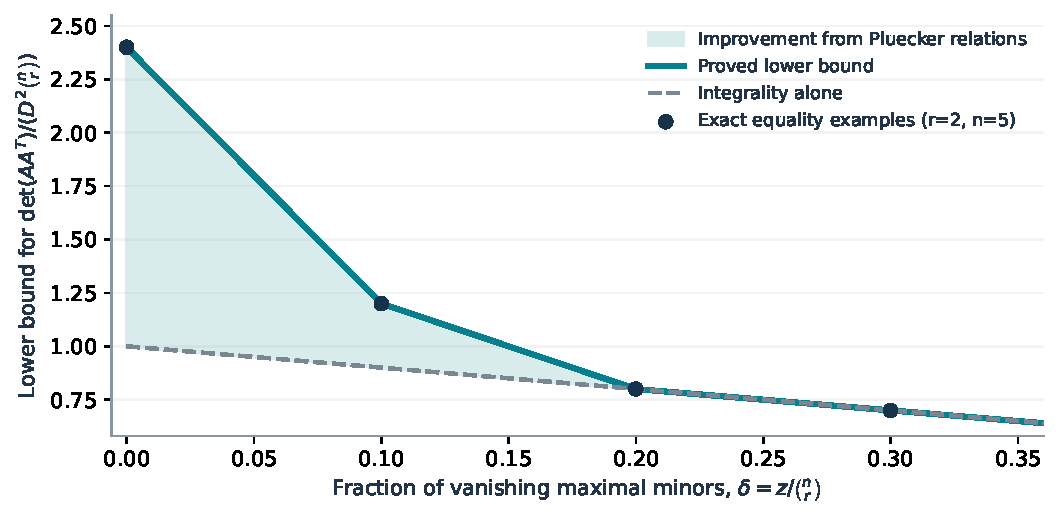
\includegraphics[width=.85\linewidth]{figures/determinant_bound.pdf}
\caption{The proven determinant lower bound as a function of the
fraction of vanishing maximal minors. The marked equality examples
have $n=5$ and $r=2$; the curve is a universal lower bound, not a
claim of optimality for every fixed dimension and zero count.}
\label{fig:det-bound}
\end{figure}

\begin{corollary}[A quantitative obstruction to short integral columns]
\label{cor:det-energy}
Under the hypotheses of Theorem~\ref{thm:determinant}, put
$E=\sum_{j=1}^n\|A_j\|^2$ and
$F=\max\{N-z,8N/5-4z,12N/5-12z\}$. Then
\[
 E\ge rD^{2/r}F^{1/r}.
\]
If every maximal minor is nonzero and every column has length at
most $H$, necessarily
\[
 \left(\frac{nH^2}{r}\right)^r\ge\frac{12}5\binom nr D^2.
\]
\end{corollary}
\begin{proof}
The positive eigenvalues of $AA^{\mathsf T}$ have sum $E$.
The arithmetic--geometric mean inequality gives
$(E/r)^r\ge\det(AA^{\mathsf T})$. Apply
Theorem~\ref{thm:determinant}, and use $E\le nH^2$ in the last case.
\end{proof}

This corollary makes the methodological connection precise: common
determinantal divisibility, many independent column subsets, and small
total squared length impose competing requirements. It does not by
itself improve the repository's RH proof. Such an application would
require matching its forms and lattices to the matrix hypotheses and
normalization used here.

The closest literature located concerns generic integer matrices with
bounded largest maximal minor and their maximal number of columns
\cite{generic2023,generic2025}. In particular, the weaker fact that a
generic two-row five-column integer matrix must have a minor of absolute
value at least three is already known. The proposed contribution here
is the aggregate sum-of-squares inequality, its explicit dependence on
vanishing minors, and the local proof with equality examples. A targeted
literature search did not locate this formulation; it does not establish
priority. The supplied exact-arithmetic script verifies all five
displayed examples, independently of the human proof above.
